%%%%%%%%%%%%%%%%%%%%%%%%%%%%%%%%%%%%%%%%%%%%%%%%%%%%%%%%%%%%%%%%%%%%%%%%%%%%%%%%
% input_validation.tex
%%%%%%%%%%%%%%%%%%%%%%%%%%%%%%%%%%%%%%%%%%%%%%%%%%%%%%%%%%%%%%%%%%%%%%%%%%%%%%%%
\chapter{Partial Disappearance Event Classification}
\label{sec:BDT}
Unlike the total disappearance region, where rejecting standalone muons and limiting calorimeter energy is sufficient to control muon backgrounds, the partial disappearance region must separate potential signal events based on a large number of input features, often with subtle correlations between them.
The primary distinguishing feature of signal events in this region is a large mismatch in the energy of the nearest standalone muon and the selected probe track, but the requirement that the standalone muon have less than 30$\%$ of the probe track still leaves several thousand background events.

Primarily caused by poorly reconstructed standalone muons, these backgrounds often have poorer fit qualities, CSC hits closer to the projected track, and larger HCAL energy deposits.
These effects are not fully independent.
For instance, muons with large HCAL energy may have genuine track deflection from SM scattering, so their fit qualities will be better.
Similarly, muons with poor quality fits will often have several missing CSC hits, allowing poor standalone muons with large energy differences to be reconstructed.

Signal events often have differences in the $\phi$ of the standalone muon which are correlated with the track charge, as the lower energy deflected muons have additional curvature in the magnetic field.
Signal events may also have significant CSC hit offsets due to the angular scatter caused by \dbrem, or missing energy in several HCAL depths from muons deflecting outside of their acceptance.

To take advantage of the wide variety of weak input separators available in this region, a Boosted Decision Tree (BDT) classifier is used to reduce these inputs to one classification variable.

\section{Boosted Decision Trees}
Boosted decision trees are a type of supervised machine learning where separate additive functions are used to map a set of inputs to a single output.
Each individual function consists of a single 'tree', where input data is split recursively over a series of 'depths'. 
The depths are made of 'nodes', where the data is split based on a selection applied to some input variables, and 'leaves', a terminal value of the tree where a value is output.
Each node is chosen to optimize the information gained by the split made, and the tree continues until the maximum depth is reached or no further information is gained.

The "boosting" originates from the method used to produce many input trees and combine their outputs \cite{GradBoost}. 
As it is normally impossible to create all potential tree structures, trees are generated iteratively by starting from a single leaf and adding branches which minimize the "loss function", which is some function used to quantify the distance between the true and predicted value.
In this analysis, the loss function is chosen to be a binary logistic function,

\begin{equation}
	\label{binLogFunc}
	L = - \frac{1}{N} \sum_{i=1}^{N} y_i log(p(y_i)) + (1-y_i) log(1-p(y_i))
\end{equation} 

where N is the total number of training events, $y_i$ is the true value of each point with zero for background and one for signal, and $p(y_i)$ is the output score for that point.
The binary logistic loss function is small for predictions which are close to the true value, and increases exponentially for predictions which are far from the true value to increase the penalty for incorrect classification.

Each tree is then given a weight according to its accuracy and combined to produce a continuous output score from zero to one, with events near zero being the most background-like and events near one being the most signal-like. 
After each step of optimizing the tree weights, the training data is re-weighted to increase the importance of events that are more frequently misclassified in order to more quickly approach the strongest classification.
The tree optimization and re-weighting is then continued for several iterations in order to minimize an objective function consisting of the loss function and a regularization function, which reduces overtraining by penalizing the complexity of the trees used.

The main advantage of tree boosting is that it allows many weak classifiers in the individual trees to be combined into one strong classifier using the ensemble output score.
In this analysis, a "Gradient" BDT was used, provided by the XGBoost framework \cite{XGBoost} interfaced with Scikit-learn \cite{scikit}. 

The BDT is trained using only the signal masses and DY MC background, as the preselection and standalone muon requirements alone are significant enough to reduce $\mu+X$ events to manageable levels. 

\section{Inputs}
There are 21 event variables which are used as inputs to the BDT, which can be grouped into five categories.

The first are variables related to the probe track kinematics. 
The $p_t$, $\eta$, $\phi$, and charge of the probe track are used in order to allow the network to encode effects which may be local to certain regions of the detector.
As the CSCs have known gaps in particular depths and regions of poor reconstruction, these variables can help identify tracks which may be expected to have lower quality.

Second are the standalone muon kinematics, specifically its energy and $\chi^{2}$ %\Cref{fig:staKin}).
The $\chi^{2}$ of the standalone muon fit is used to measure its quality, and helps to separate muons with genuine energy loss from those with poor fits.
The overall standalone muon energy is used in addition to the difference in standalone muon and probe track energy in case there are energy-dependent factors that may be lost when using only the relative measure.

%\begin{figure}[htpb]
%	\label{fig:staKin}
%	\includegraphics[width=0.45\textwidth]{figures/}
%	\hspace{0.01\textwidth}
%	\includegraphics[width=0.45\textwidth]{figures/}
%	\caption[short caption]{long caption}
%\end{figure}

The third category are the CSC segment distances.
In each CSC station, the minimum $\Delta$R is measured from each CSC segment to the projected probe track at its position of closest approach to that segment.
Signal events often see finite differences in these CSC hit differences, while background events often have very close CSC hits in every station or have several stations with no nearby segments resulting in a poor fit and significant mismeasured energy.

Fourth, the difference between the standalone muon and the probe track in energy, $\Delta$R, and $\Delta \phi$ are used.
Signal events are have significantly lower energy standalone muons from energy loss to the \aprime, as well as larger $\Delta$R from angular deflection in \dbrem and additional curvature in the magnetic field.
To help distinguish angular changes caused by energy loss, the $\Delta \phi$ between the standalone muon and probe track is multiplied by the track charge, as differences due to random scatters and poor reconstruction should have no correlation between the charge and $\Delta \phi$.

Lastly, the HCAL energy in each depth along the probe trajectory is used to identify events with high energy deposits corresponding to SM processes, or multiple low energy deposits corresponding to potential signal events.
The number of depths traversed by any given muon depends on its position in HCAL.
To accomodate this, projected tracks which do not pass through a given depth in HCAL are assigned an energy of -1. 

\section{Optimization}
A significant difficulty in training the partial region BDT is the imbalance between signal and background events. 
Because \dbrem is expected to be a rare process, many more background events are expected than signal events, and the background rejection rate must be prioritized over signal selection efficiency.

To represent this, signal events are given reduced weights to replicate their lower relative rate and increase the importance of background rejection.
Prior to optimization of the other parameters, a scan of this signal weight is made and the value which produces the strongest signal limit is selected.
To reduce the necessary validation and simplify the network, each signal mass is combined into one training input and weighted to give equal importance to each mass.

The internal parameters of the BDT are chosen using a randomized search, where each parameter is sampled from a flat distribution of possible values for a large number of trials.
To reduce the impact of overtraining in this parameter optimization, the training data is split into five randombly sampled independent subsets called \emph{folds}.
Five separate testing and training combinations sets are then defined, each with the test set as one fold and the training set as the other four.

Five separate BDTs are then trained using these datasets, and the average weighted mean squared error of the five BDTs is used as the figure of merit in the randomized parameter search.
By selecting the parameters with the smallest average mean squared error, the optimum parameters can be chosen by using the entire dataset to test the performance, as every event has a BDT which did not use it as training data, reducing the potential bias caused by the testing selection.

The parameters which are optimized are the number of trees, the maximum tree depth, the fraction of each training sample used, the weighting factor of each new tree, the loss reduction required to create new leaves, the fraction of input features used in each tree, the minimum weight in each node, and the strength of the regularization terms used in the objective function.

\section{Validation}
\label{sec:BDTvalid}
Two control regions are used to validate the performance of the BDT on background events, one consisting of probe tracks with large HCAL isolations ($>$\SI{30}{\giga\eV}), and one consisting of events with BDT scores less than 0.7. 
The HCAL energy requirement tends to select for muons which have had hard SM scatters within the detector, and thus have more signal-like features in the muon chambers and more background-like features in the HCAL.

Events with poor HCAL isolation also select for $\mu+X$ backgrounds at a much larger rate than in the signal region.
In order to estimate their impact, data events with the equivalent HCAL isolation requirement and same-sign tag/probe pairs are used.
Though these events do not contain $\mu$+X backgrounds from charge correlated processes, they can be used to provide an estimate for the distribution and relative scale of the overall backgrounds.

The distributions of the standalone muon $\Delta$E/E, $\chi^{2}$, and $\Delta\phi$ are shown in \Cref{fig:BDTstavalid}. 
Differences between data and MC are observed for some regions of all three variables, particularly at low muon energy, high standalone muon reduced $\chi^{2}$, and $\Delta\phi$ with magnitude near 0.2. 

\begin{figure}[htbp]
	\centering
	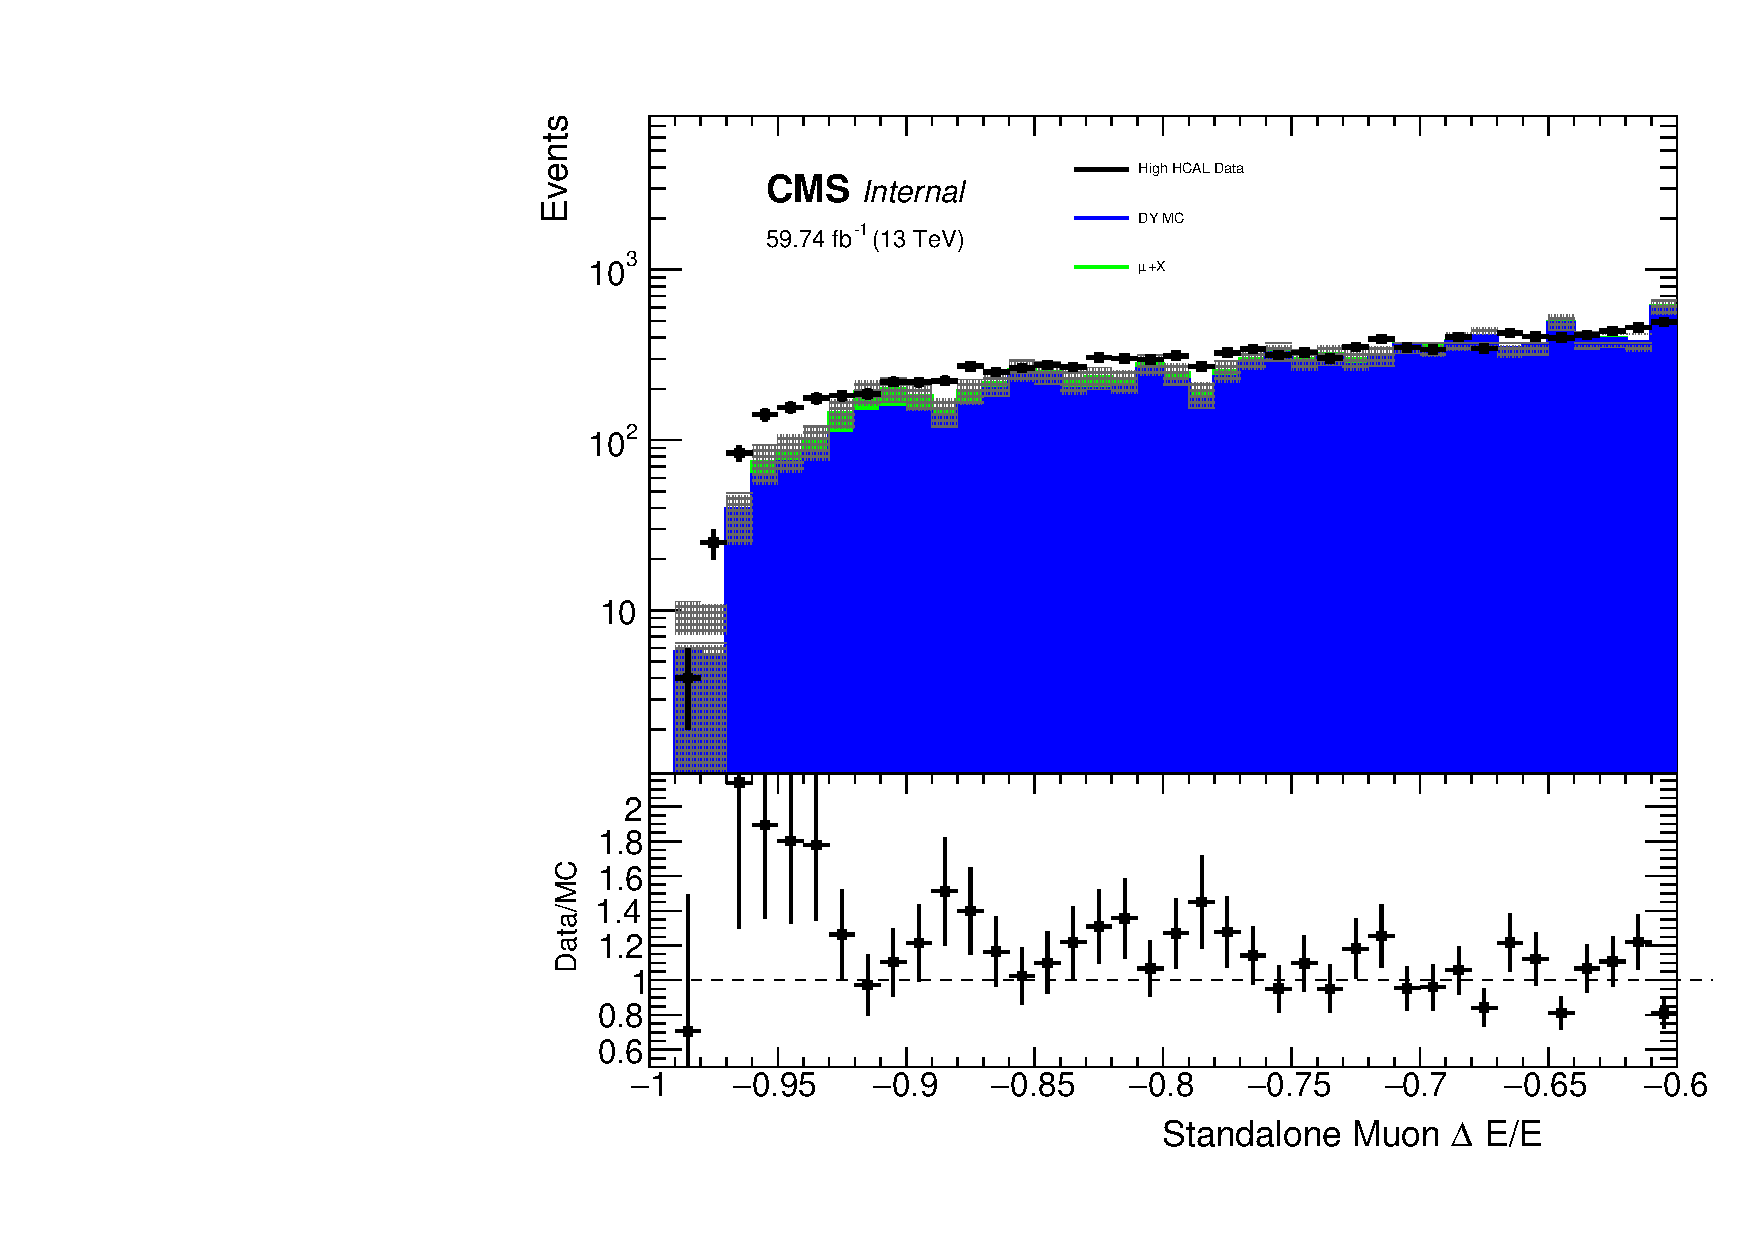
\includegraphics[width=0.45\textwidth]{figures/standaloneMuonValidation.pdf}
	\hspace{0.01\textwidth}
	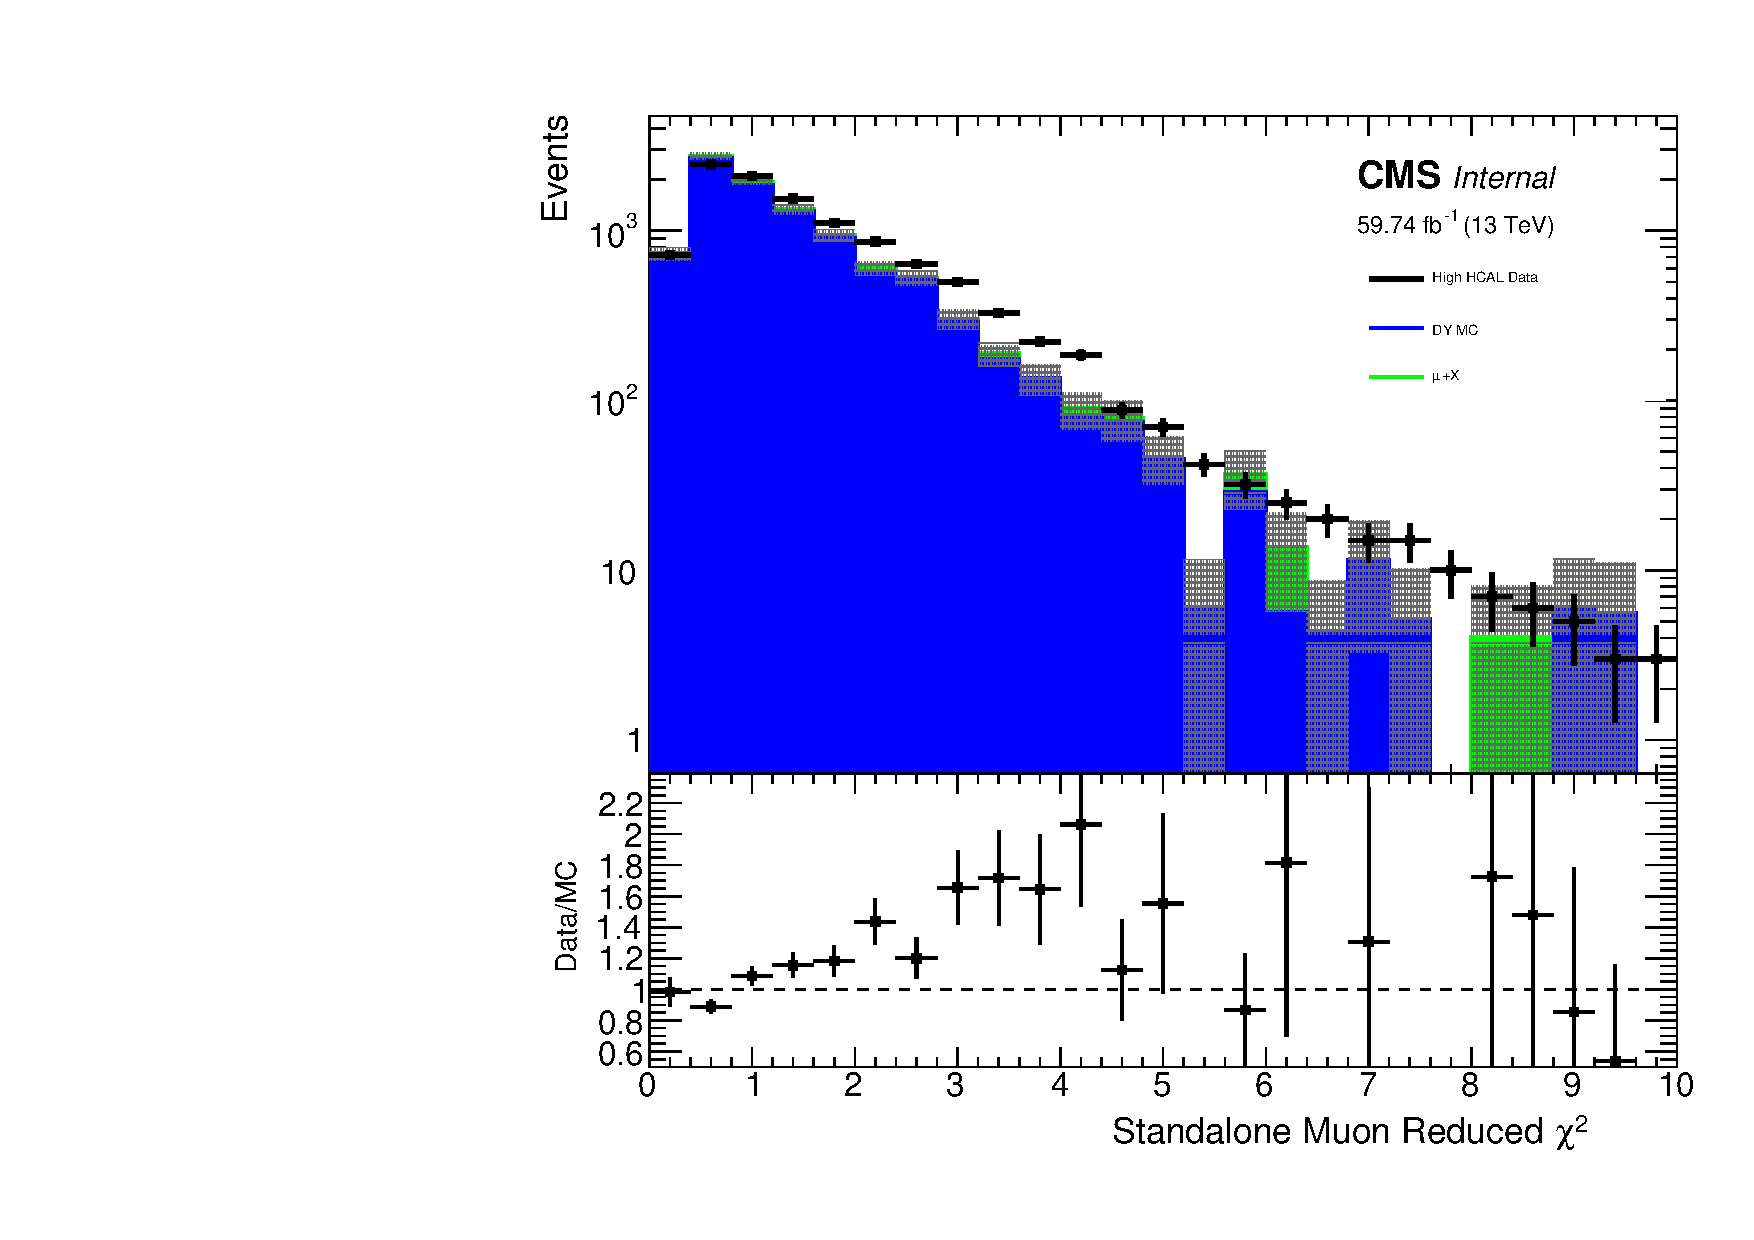
\includegraphics[width=0.45\textwidth]{figures/standaloneMuonChiValidation.pdf}
	\vspace{0.01\textwidth}
	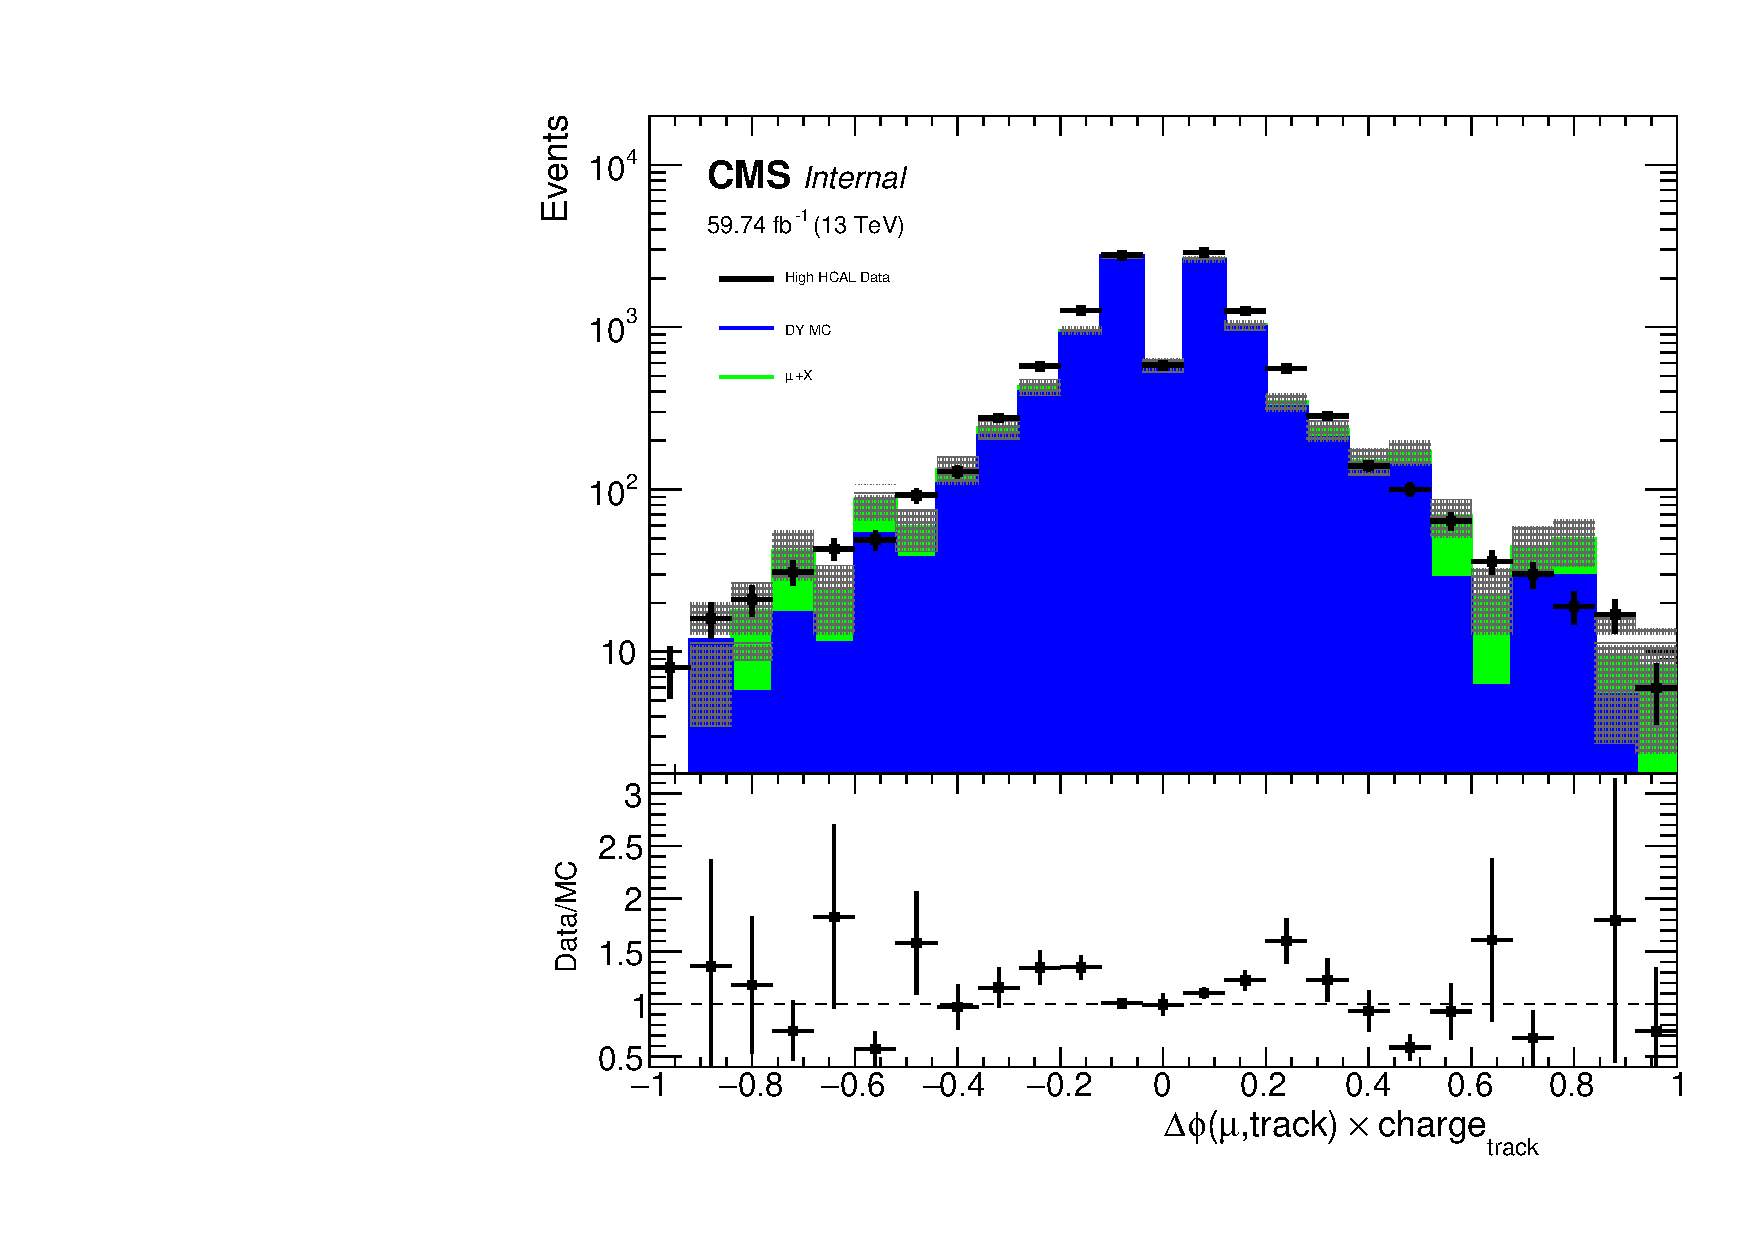
\includegraphics[width=0.45\textwidth]{figures/standaloneMuonPhiValidation.pdf}
        \caption[Standalone Muon Validation]{Standalone muon variables used as inputs to the partial region BDT measured in the high HCAL energy control region. Discrepancies are present in events with very low standalone muon $\Delta$E/E, large reduced $\chi^{2}$, and $\Delta\phi$ of $~|$0.2$|$.}
        \label{fig:BDTstavalid}
\end{figure}

The distributions of the distance to the nearest CSC hit in each muon station is presented in \Cref{fig:BDTcscvalid}. 
Some differences between MC and data are observed in the CSC $\Delta$R distributions as well. 
As with the tag-muon aligned segments, station 1 has significant excesses of events with large $\Delta$R to the nearest hit and no nearby hits, while the other three depths have better overall agreement but overestimate the rates of events with intermediate $\Delta$R to the nearest in the range of 0.1 to 2.

\begin{figure}[htbp]
	\label{fig:BDTcscvalid}
	\centering
	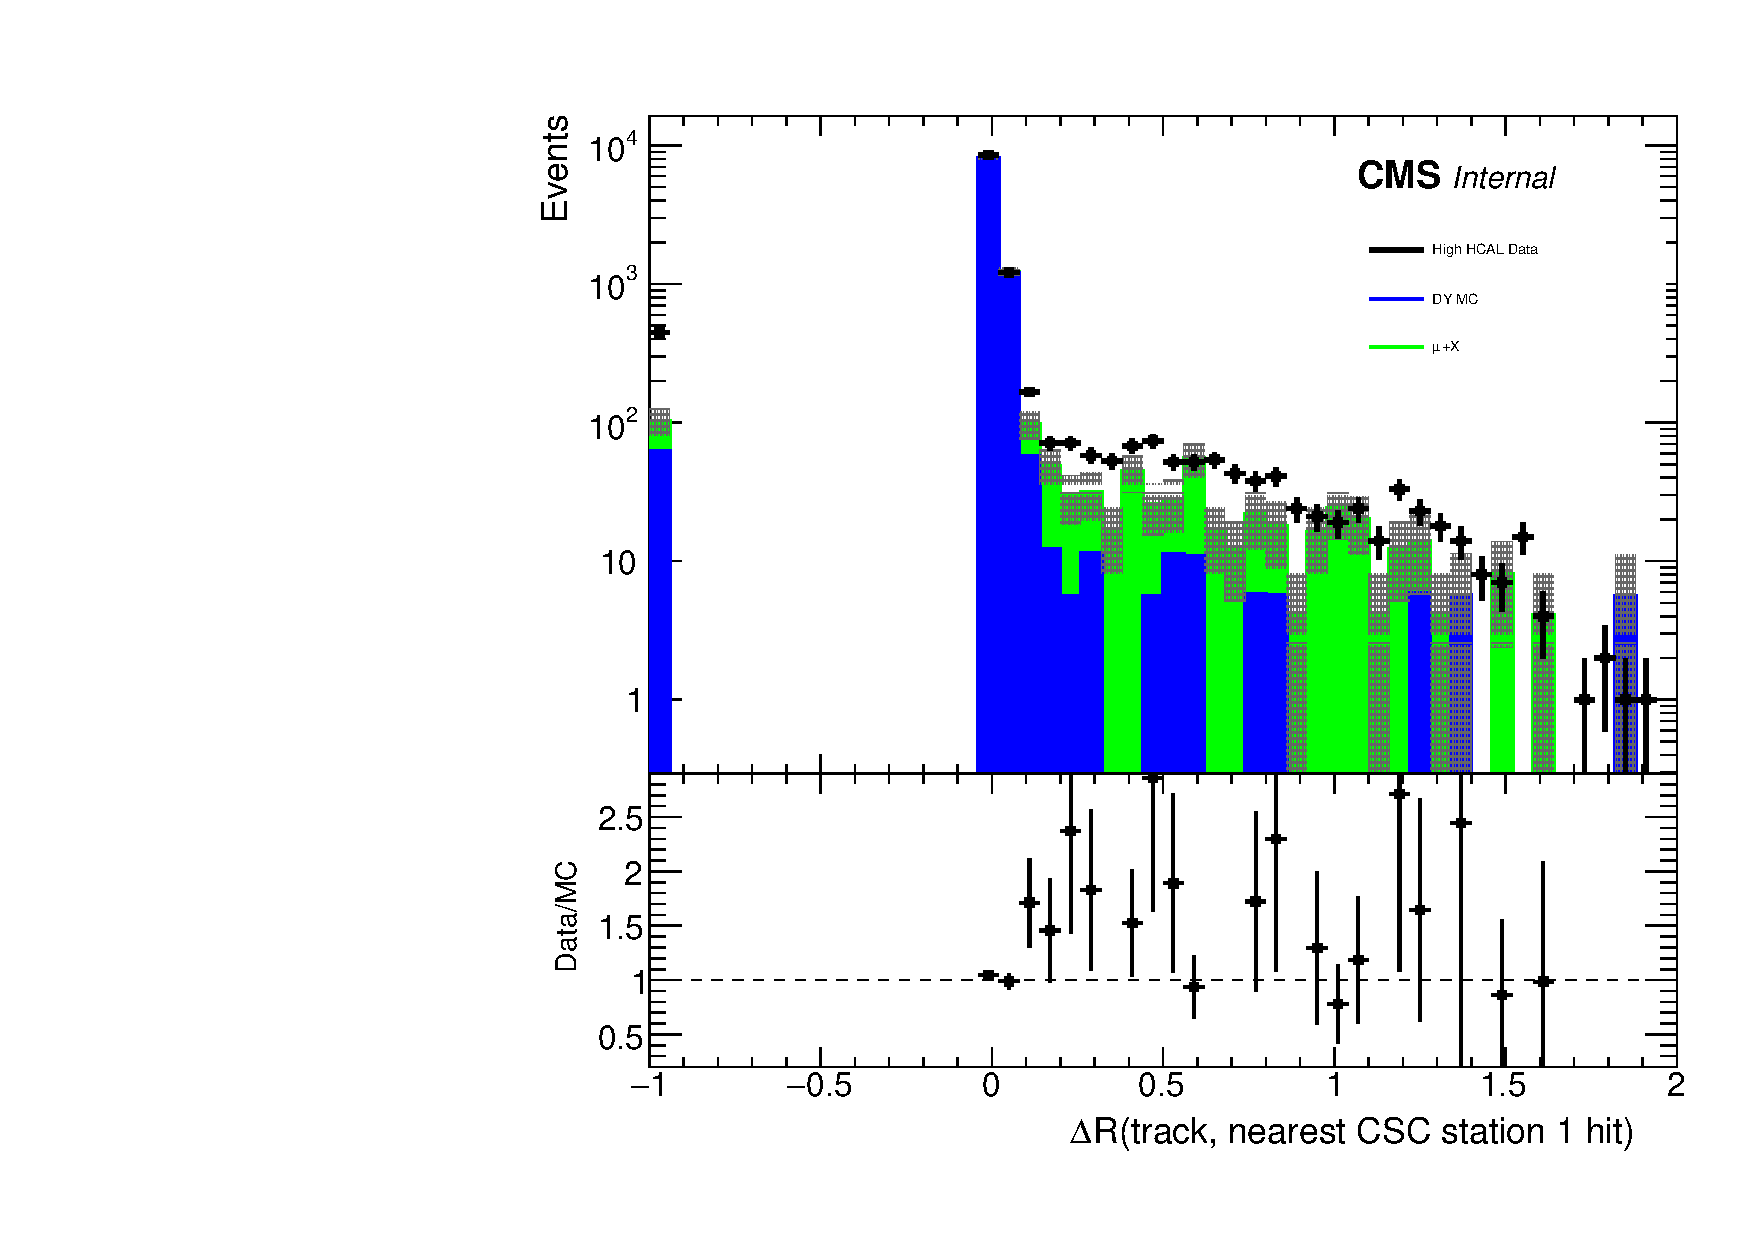
\includegraphics[width=0.45\textwidth]{figures/highHcal_cscDr_station0.pdf}
	\hspace{0.01\textwidth}
	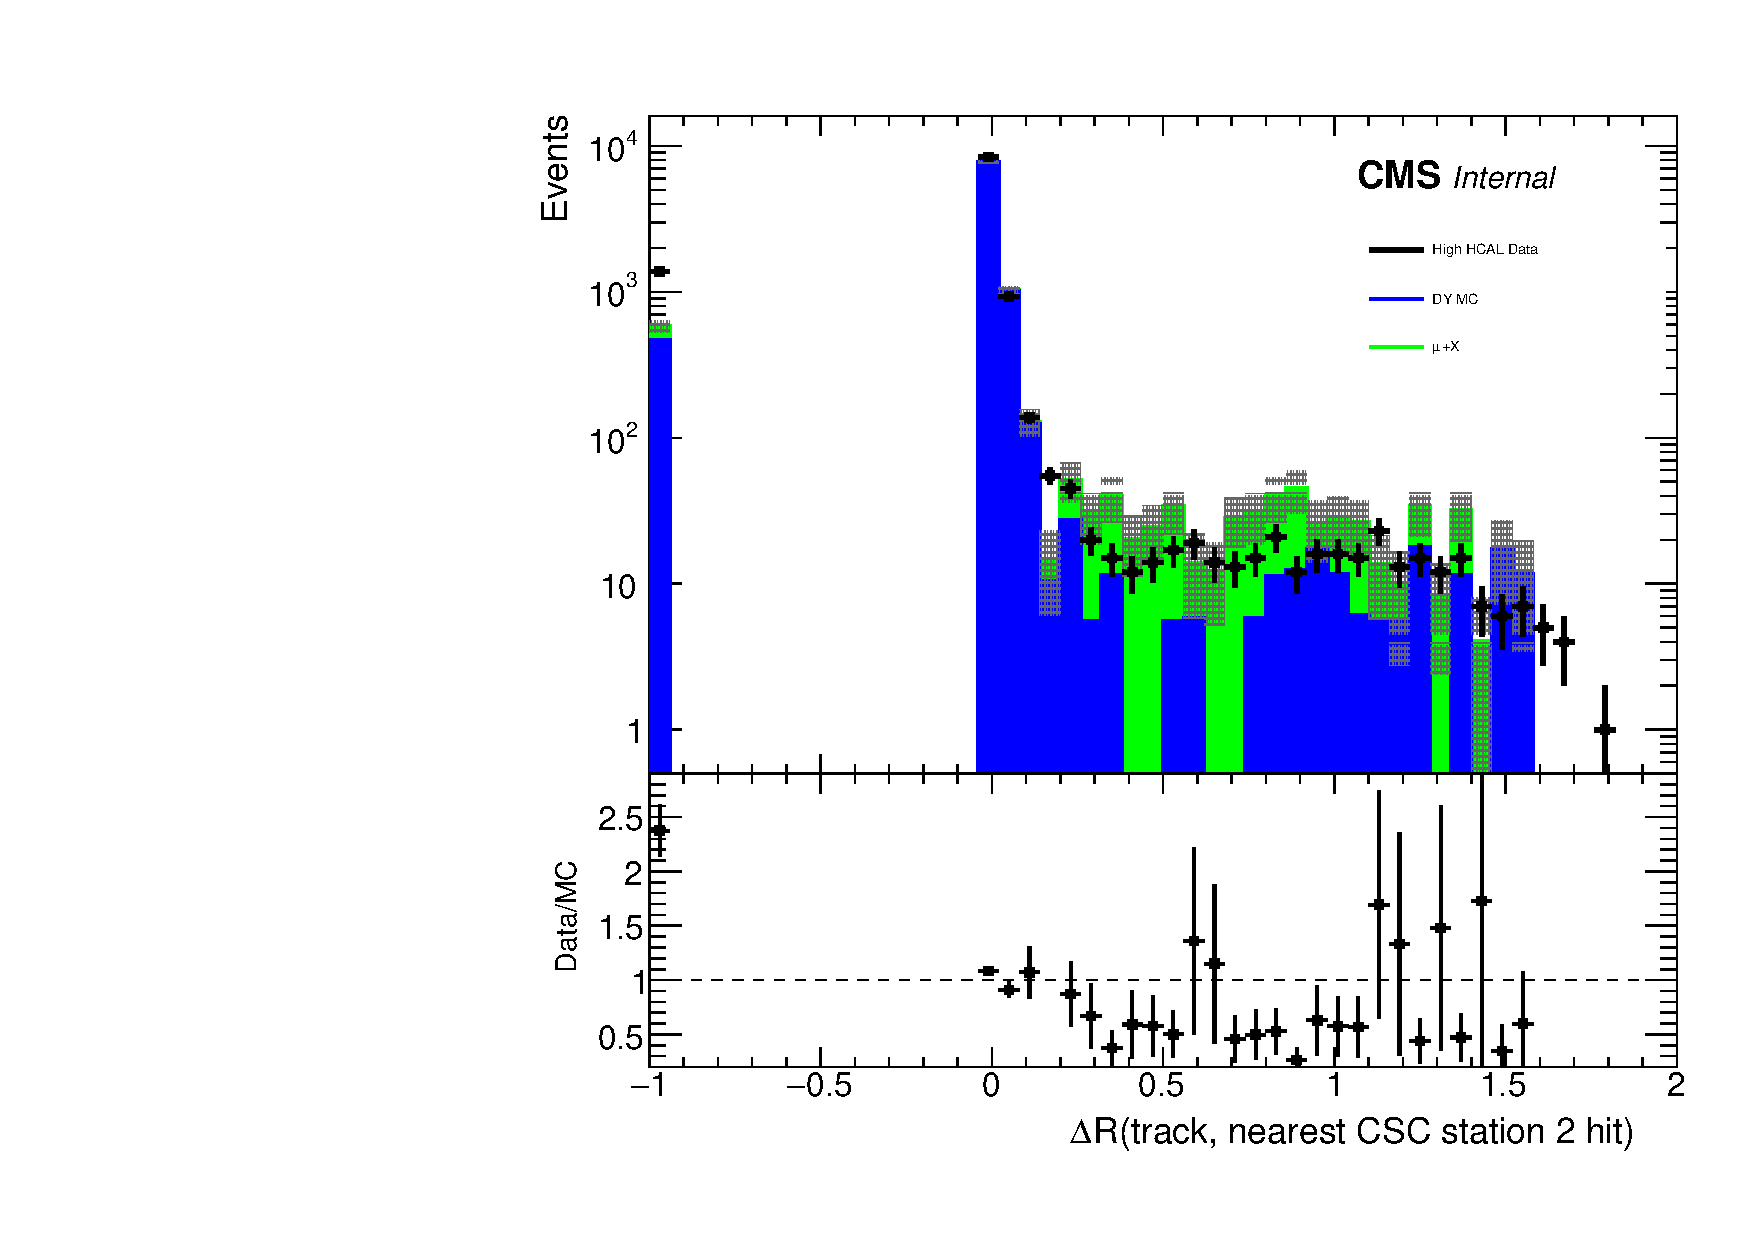
\includegraphics[width=0.45\textwidth]{figures/highHcal_cscDr_station1.pdf}
	\vspace{0.01\textwidth}
	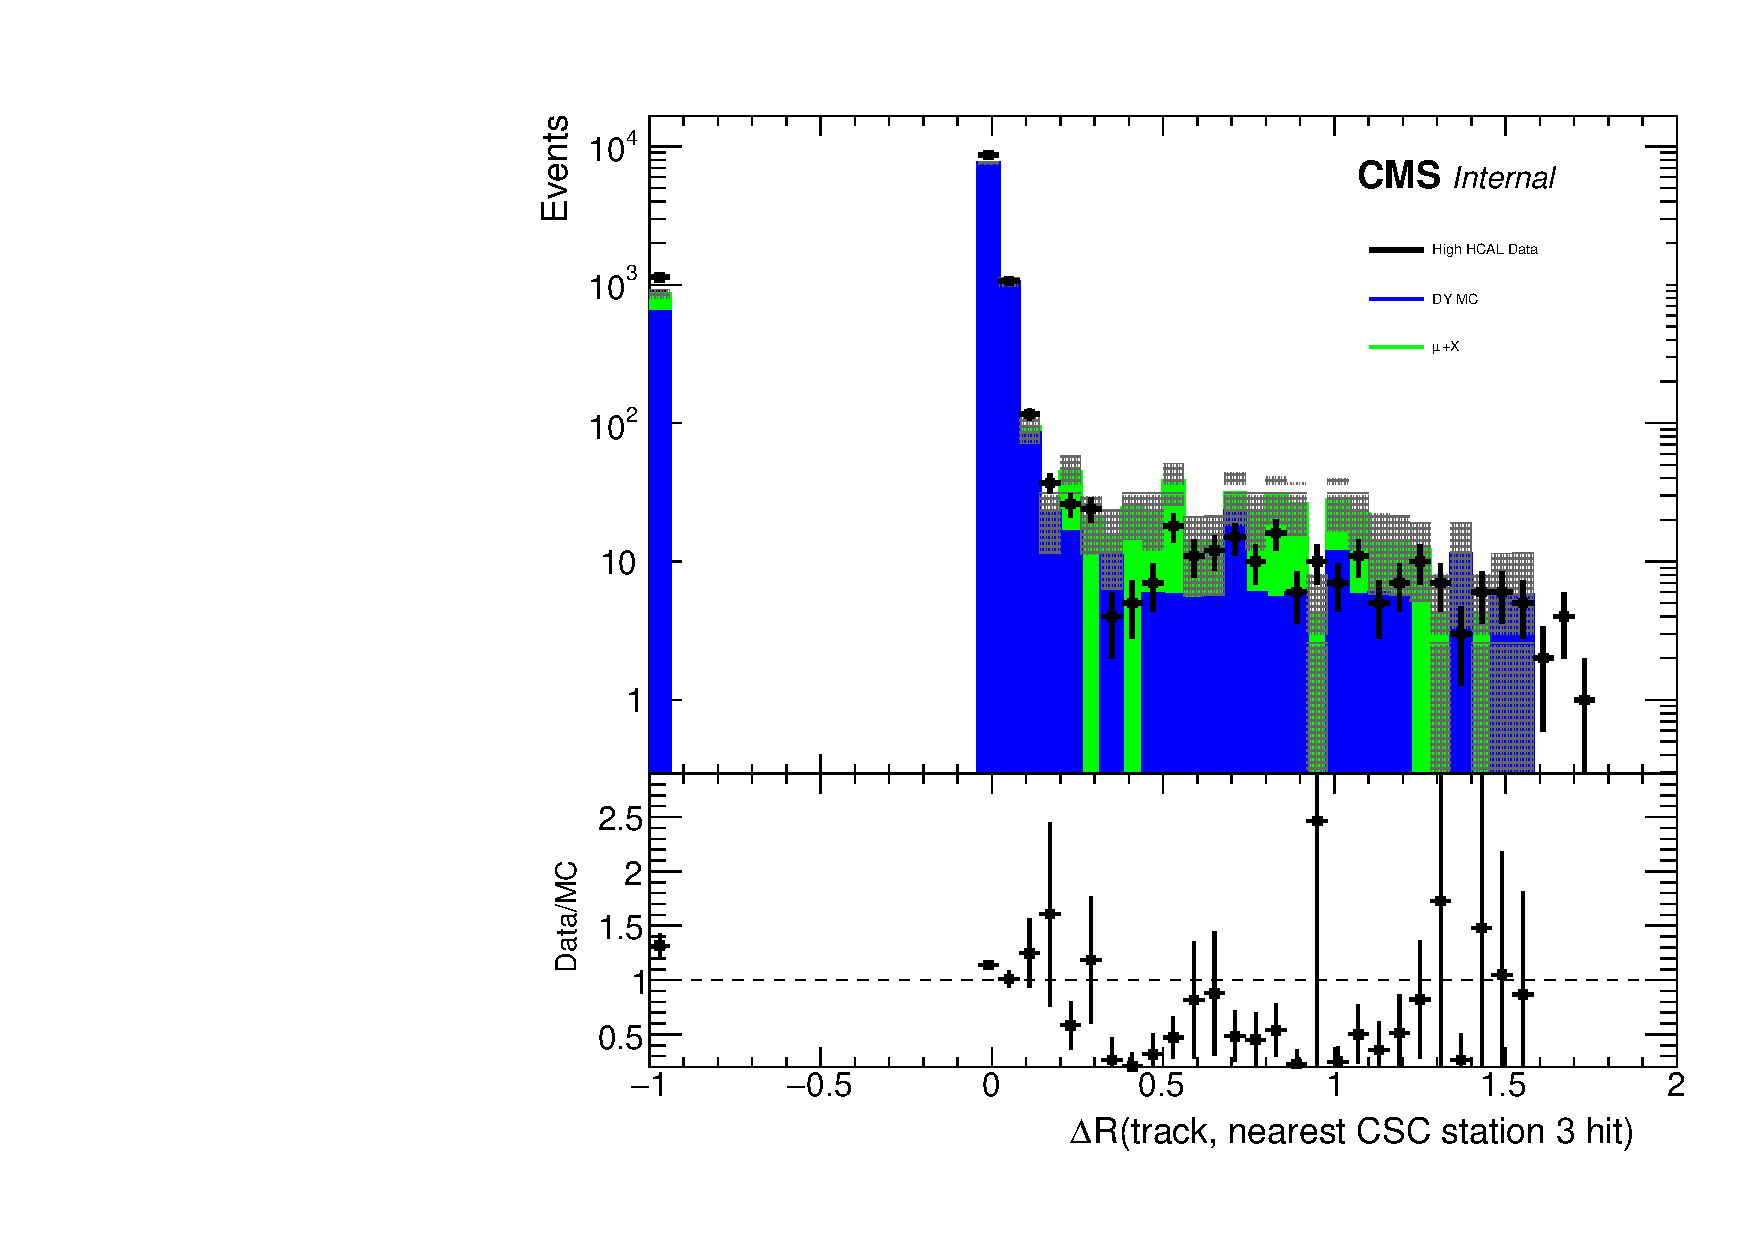
\includegraphics[width=0.45\textwidth]{figures/highHcal_cscDr_station2.pdf}
	\hspace{0.01\textwidth}
	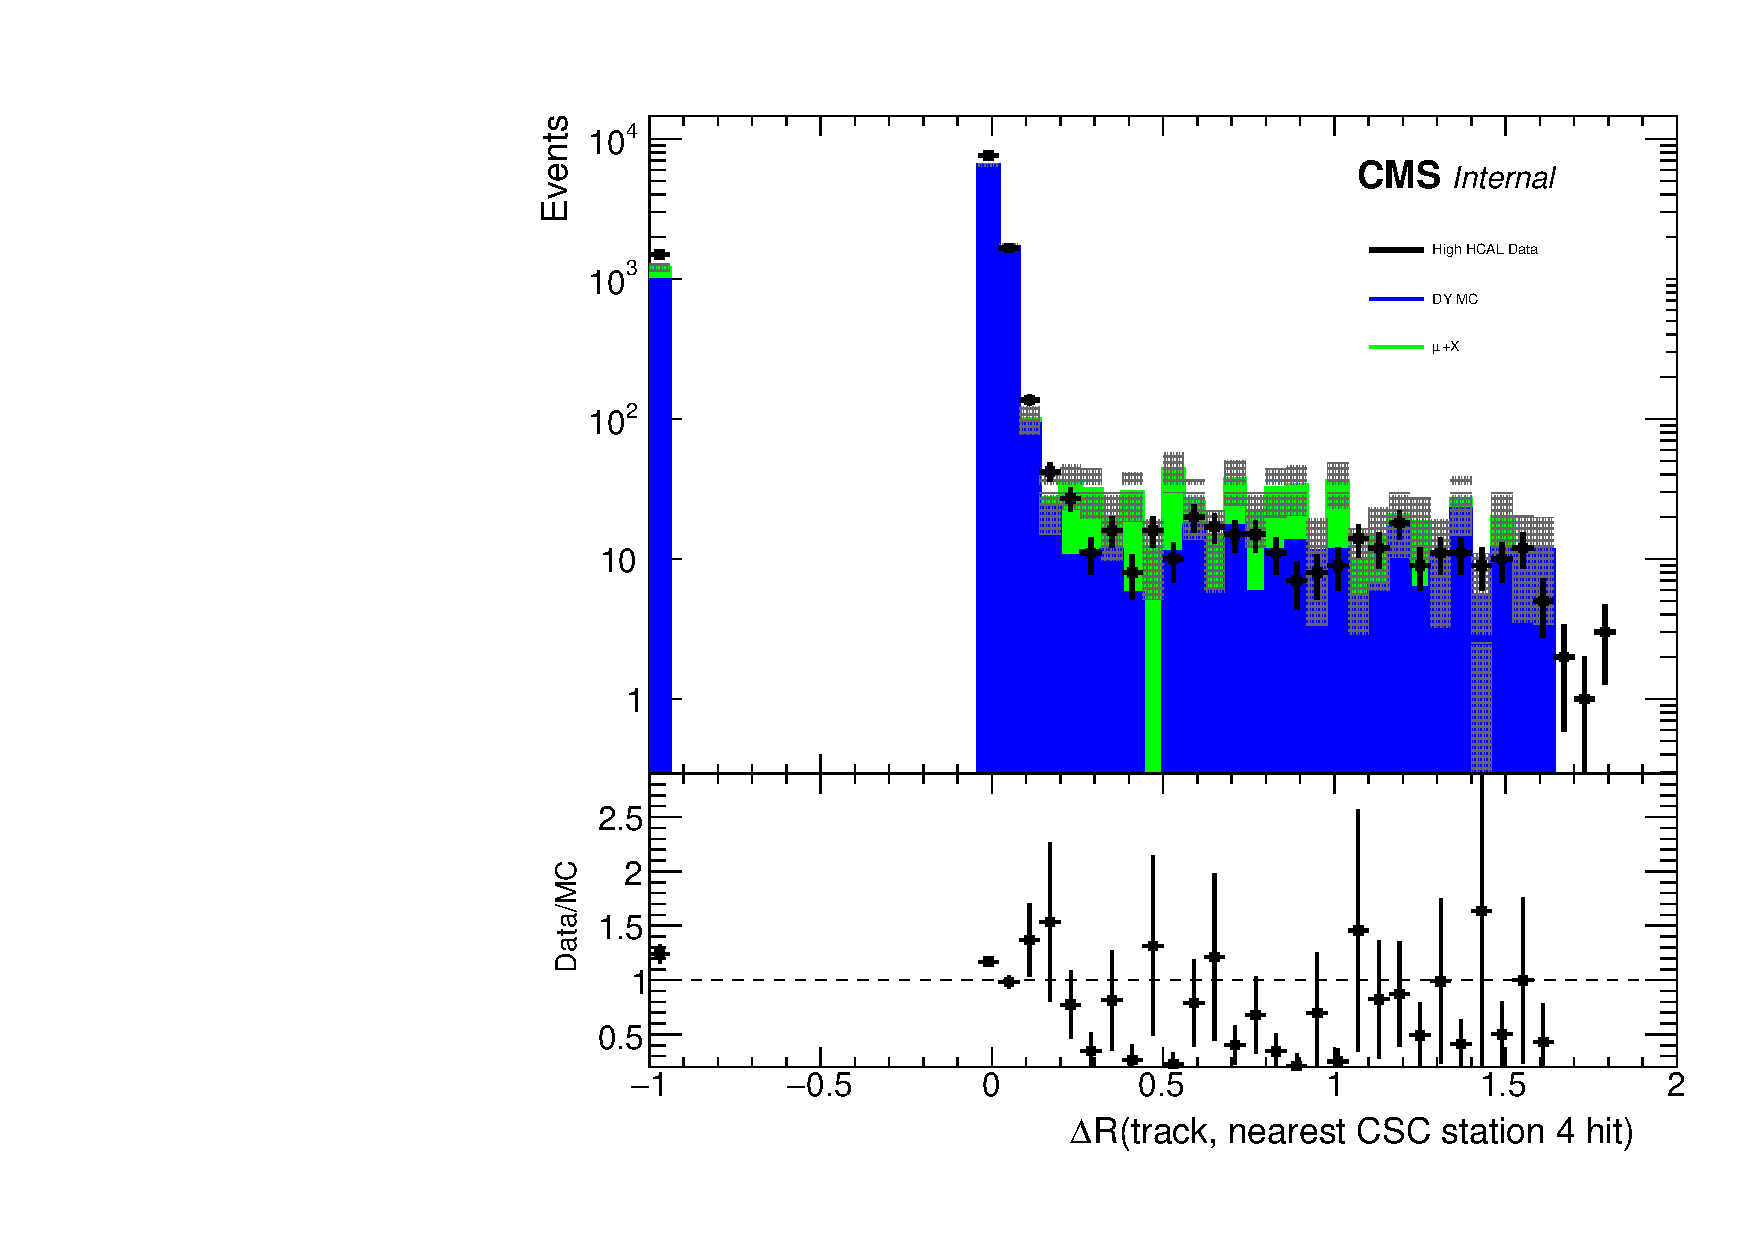
\includegraphics[width=0.45\textwidth]{figures/highHcal_cscDr_station3.pdf} 
        \caption[CSC Segment Validation]{The distance to the nearest CSC segment in each station measured along the probe track trajectory for partial disappearance events in the high HCAL energy control region. Events with no CSC hits in a station within $\Delta$R of 2 are assigned a value of -1.}
\end{figure}

Despite these modeling differences, the BDT scores of events in this region do not see substantial differences between data and MC (\Cref{fig:BDTscorevalid}).
This is likely due to counteracting influences from the poorly modeled features, and the relatively small absolute event rates in these regions. 
Events with more missing CSC hits will appear more signal-like due to the potential for lower reconstructed standalone energy and larger $\Delta$R, but also have correspondingly higher $\chi^{2}$, reducing their output scores.
As expected, the region is relatively shifted to higher BDT scores than the overall DY background due to the more signal-like event features in this region produced by energy loss to standard model processes in the HCAL. 

\begin{figure}[htbp]
	\label{fig:BDTscorevalid}
	\centering
	%\includegraphics[width=0.6\textwidth]{figures/highHcal_BDTScore.pdf}
        \caption[BDT Validation in the High HCAL Energy Control Region]{The distribution of BDT scores for data and DY MC events in the high HCAL control region.}
\end{figure}

Because of the significant difference in event features between the signal region and the high-HCAL control region, these comparisons cannot be used to directly derive scale factors to correct MC. 
Instead, the potential impact of these variation can be estimated by adjusting MC features to match data within the control region and testing the resulting impact on the output BDT score.
As applying all potential corrections simultaneously may introduce counter-acting effects, the relative scale of these uncertainties is estimated by individually varying the most impactful variables.

To perform this, scale factors are derived from the ratio of the CSC hit distances by taking the ratio of the data and MC plots in each depth. 
These scale factors are then applied to DY MC in the signal region as a function of $\Delta$R in each depth and the magnitude of the resulting change in the background acceptance is applied as an overall uncertainty on the DY background prediction in the partial disappearance region. 
The shift in the overall DY BDT distribution with the CSC scale factors applied can be seen in \Cref{fig:BDTsfvalid}.

\begin{figure}[htbp]
	\label{fig:BDTsfvalid}
	\centering
	%\includegraphics[width=0.6\textwidth]{figures/highHcal_cscSF.pdf}
        \caption[BDT Score Variance with Applied CSC Scale Factors]{The distribution of BDT output scores for DY Mc events with and without CSC scale factors applied.}
\end{figure}

In the signal region (BDT Score$>0.98$), the application of the scale factors produces 8$\%$ fewer DY events, which is included as an overall systematic uncertainty on the rate of expected DY background in the partial disappearance region. 

In contrast to the high-HCAL energy region, events with low BDT scores (BDT score $<0.7$) contain background-like features in both the CSCs and HCAL, and can be used to validate the simulation of the DY backgrounds as well as the performance of the BDT on these events.
In intial studies of this region, significant differences were observed in several features related to the standalone muons, with excess events showing large $\Delta$R to the nearest standalone muon, low standalone muon energy, and large trajectory change between the probe track and the nearest standalone muon.

In addition, large differences in the overall normalization were observed between the data events and the expected rate of DY backgrounds, with nearly twice as many events selected as expected.
Through study of these anomalous events, it was found that they correspond to cases where large differences in CSC segment position were present between the first CSC station and the later three.
These position differences cause the reconstruction of the standalone muon to produce anomalously low energy and altered trajectories, resulting in several signal-like differences in the final objects. 

Large positional differences between the first and later CSC stations is not frequently seen in signal events, as energy loss within the HCAL results in significant deflection before reaching the CSC chambers, but relatively small deflection from station to station. 
As a result, these anomalous standalone muons can be removed using quality requirements based on the $\Delta$R of the nearest CSC segments in stations two, three, and four to the position of the nearest CSC segment in station one.
After removing events with no CSC segments within $\Delta\mathrm{R}<0.04$ of the nearest CSC segment in station one, significant improvement is seen in the individual standalone muon features.
The overall normalization after this additional requirement differs on the scale of $20\%$, roughly in expectation with the combined cross section, luminosity, and selection efficiency uncertainties.

The behavior of the remaining input features in the low BDT score control region is shown in , and the resulting BDT score is shown in .
